% Created 2024-10-18 Fri 00:37
% Intended LaTeX compiler: pdflatex
\documentclass[11pt]{article}
\usepackage[utf8]{inputenc}
\usepackage[T1]{fontenc}
\usepackage{graphicx}
\usepackage{longtable}
\usepackage{wrapfig}
\usepackage{rotating}
\usepackage[normalem]{ulem}
\usepackage{amsmath}
\usepackage{amssymb}
\usepackage{capt-of}
\usepackage{hyperref}
\usepackage{parskip,darkmode}
\enabledarkmode
\usepackage{tikz}
\usetikzlibrary{positioning, calc}
\usepackage{algorithm,algpseudocode}
\author{Arnav Gupta}
\date{\today}
\title{Informed/Heuristic Search}
\hypersetup{
 pdfauthor={Arnav Gupta},
 pdftitle={Informed/Heuristic Search},
 pdfkeywords={},
 pdfsubject={},
 pdfcreator={Emacs 29.4 (Org mode 9.7.11)}, 
 pdflang={English}}
\begin{document}

\maketitle
\tableofcontents

\section{Heuristic Search}
\label{sec:org7aa712d}
Use \textbf{heuristics} to guide the search towards the goals.
\(h(n)\) is an estimate of the cost of the shortest path from node \(n\) to a goal node.
Computing the heuristic must be much easier than solving the problem.

\(h(n)\) is an \textbf{underestimate} if there is no path from \(n\) to a goal that has path length
less than \(h(n)\).
\subsection{Greedy Best-First Search}
\label{sec:org9f531f3}
Select the path whose end is closest to a goal according to the heuristic function, that is minimal
\(h\) value.
Treat the frontier as a priority queue ordered by \(h\).

\begin{center}
    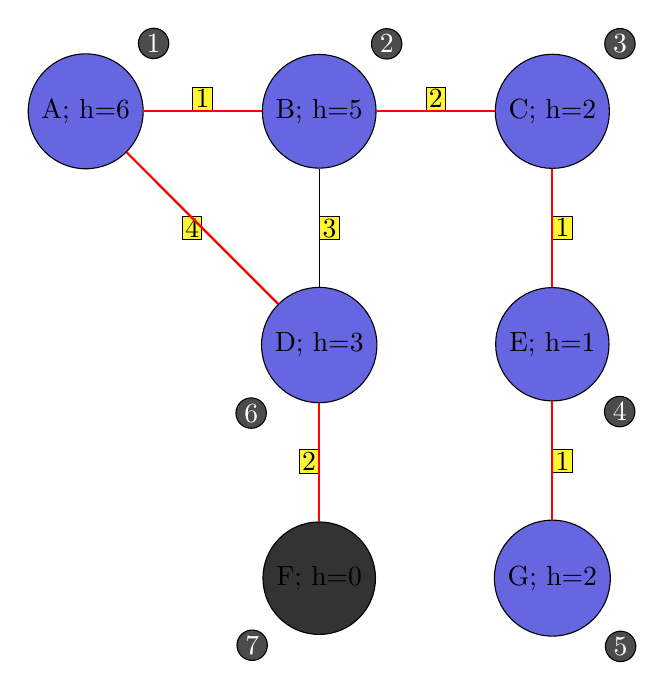
\begin{tikzpicture}[node distance=1.5cm, every node/.style={circle, draw, fill=blue!80!black!60}]
        \node (A) {A; h=6}; % Node A with heuristic 6
        \node (B) [right=of A] {B; h=5}; % Node B with heuristic 5
        \node (C) [right=of B] {C; h=2}; % Node C with heuristic 2
        \node (D) [below=of B] {D; h=3}; % Node D with heuristic 3
        \node (E) [below=of C] {E; h=1}; % Node E with heuristic 1
        \node (F) [below=of D, fill=black!80] {F; h=0}; % Goal node F highlighted with heuristic 0
        \node (G) [below=of E] {G; h=2}; % Node G with heuristic 2

        \draw (A) -- (B);
        \draw (A) -- (D);
        \draw (B) -- (C);
        \draw (B) -- (D);
        \draw (C) -- (E);
        \draw (D) -- (F);
        \draw (E) -- (G);

        % Cost labels with better visibility
        \node[draw, rectangle, fill=yellow!80, text=black, inner sep=1pt] at ($(A)!0.5!(B)$) [above] {1};
        \node[draw, rectangle, fill=yellow!80, text=black, inner sep=1pt] at ($(A)!0.5!(D)$) [left] {4};
        \node[draw, rectangle, fill=yellow!80, text=black, inner sep=1pt] at ($(B)!0.5!(C)$) [above] {2};
        \node[draw, rectangle, fill=yellow!80, text=black, inner sep=1pt] at ($(B)!0.5!(D)$) [right] {3};
        \node[draw, rectangle, fill=yellow!80, text=black, inner sep=1pt] at ($(C)!0.5!(E)$) [right] {1};
        \node[draw, rectangle, fill=yellow!80, text=black, inner sep=1pt] at ($(D)!0.5!(F)$) [left] {2};
        \node[draw, rectangle, fill=yellow!80, text=black, inner sep=1pt] at ($(E)!0.5!(G)$) [right] {1};

        % Highlight the explored edges
        \foreach \i/\j in {A/B, A/D, B/C, C/E, D/F, E/G} {
            \draw[thick, red] (\i) -- (\j);
        }

        % Indicate traversal order with black circles
        \node[draw, circle, fill=black!70, inner sep=1pt] at (A) [above right=0.2cm and 0.2cm of A] {\textcolor{white}{1}};
        \node[draw, circle, fill=black!70, inner sep=1pt] at (B) [above right=0.2cm and 0.2cm of B] {\textcolor{white}{2}};
        \node[draw, circle, fill=black!70, inner sep=1pt] at (D) [below left=0.2cm and 0.2cm of D] {\textcolor{white}{6}};
        \node[draw, circle, fill=black!70, inner sep=1pt] at (C) [above right=0.2cm and 0.2cm of C] {\textcolor{white}{3}};
        \node[draw, circle, fill=black!70, inner sep=1pt] at (F) [below left=0.2cm and 0.2cm of F] {\textcolor{white}{7}};
        \node[draw, circle, fill=black!70, inner sep=1pt] at (E) [below right=0.2cm and 0.2cm of E] {\textcolor{white}{4}};
        \node[draw, circle, fill=black!70, inner sep=1pt] at (G) [below right=0.2cm and 0.2cm of G] {\textcolor{white}{5}};
\end{tikzpicture}
\end{center}
\subsubsection{Properties of GBFS}
\label{sec:orgc5c6689}
Properties:
\begin{itemize}
\item \emph{space complexity}: exponential
\item \emph{time complexity}: exponential
\item \emph{completeness}: no, could be stuck in a cycle
\item \emph{optimality}: no, may return sub-optimal path first
\end{itemize}
\subsection{Heuristic Depth-First Search}
\label{sec:org8c8c8e4}
Do a DFS but add paths to the stack ordered by \(h\).

Same properties as DFS.
\section{A* Search}
\label{sec:orgdb09d56}
Use both path cost and heuristics.
The sum of the path cost and heuristic from the end of the path to the goal is the \textbf{total path cost}.

Treats the frontier as a priority queue ordered by this sum.
Always selects the node on the frontier with the lowest estimated distance from the start to a goal node
constrained to go via that node.

\begin{center}
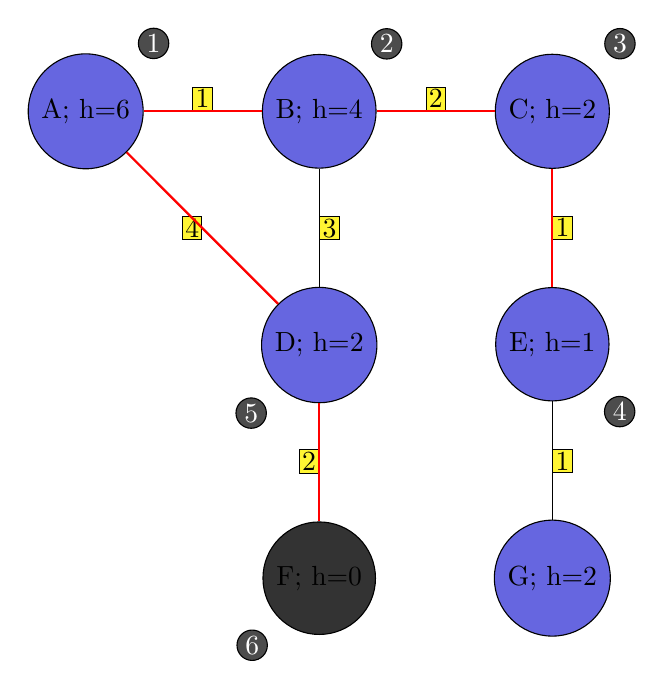
\begin{tikzpicture}[node distance=1.5cm, every node/.style={circle, draw, fill=blue!80!black!60}]
        \node (A) {A; h=6}; % Node A with heuristic 6
        \node (B) [right=of A] {B; h=4}; % Node B with heuristic 4
        \node (C) [right=of B] {C; h=2}; % Node C with heuristic 2
        \node (D) [below=of B] {D; h=2}; % Node D with corrected heuristic 2
        \node (E) [below=of C] {E; h=1}; % Node E with heuristic 1
        \node (F) [below=of D, fill=black!80] {F; h=0}; % Goal node F highlighted with heuristic 0
        \node (G) [below=of E] {G; h=2}; % Node G with heuristic 2

        \draw (A) -- (B);
        \draw (A) -- (D);
        \draw (B) -- (C);
        \draw (B) -- (D);
        \draw (C) -- (E);
        \draw (D) -- (F);
        \draw (E) -- (G);

        % Cost labels with better visibility
        \node[draw, rectangle, fill=yellow!80, text=black, inner sep=1pt] at ($(A)!0.5!(B)$) [above] {1};
        \node[draw, rectangle, fill=yellow!80, text=black, inner sep=1pt] at ($(A)!0.5!(D)$) [left] {4};
        \node[draw, rectangle, fill=yellow!80, text=black, inner sep=1pt] at ($(B)!0.5!(C)$) [above] {2};
        \node[draw, rectangle, fill=yellow!80, text=black, inner sep=1pt] at ($(B)!0.5!(D)$) [right] {3};
        \node[draw, rectangle, fill=yellow!80, text=black, inner sep=1pt] at ($(C)!0.5!(E)$) [right] {1};
        \node[draw, rectangle, fill=yellow!80, text=black, inner sep=1pt] at ($(D)!0.5!(F)$) [left] {2};
        \node[draw, rectangle, fill=yellow!80, text=black, inner sep=1pt] at ($(E)!0.5!(G)$) [right] {1};

        % Highlight the explored edges
        \foreach \i/\j in {A/B, A/D, B/C, C/E, D/F} {
            \draw[thick, red] (\i) -- (\j);
        }

        % Indicate traversal order with black circles
        \node[draw, circle, fill=black!70, inner sep=1pt] at (A) [above right=0.2cm and 0.2cm of A] {\textcolor{white}{1}};
        \node[draw, circle, fill=black!70, inner sep=1pt] at (B) [above right=0.2cm and 0.2cm of B] {\textcolor{white}{2}};
        \node[draw, circle, fill=black!70, inner sep=1pt] at (D) [below left=0.2cm and 0.2cm of D] {\textcolor{white}{5}};
        \node[draw, circle, fill=black!70, inner sep=1pt] at (F) [below left=0.2cm and 0.2cm of F] {\textcolor{white}{6}};
        \node[draw, circle, fill=black!70, inner sep=1pt] at (C) [above right=0.2cm and 0.2cm of C] {\textcolor{white}{3}};
        \node[draw, circle, fill=black!70, inner sep=1pt] at (E) [below right=0.2cm and 0.2cm of E] {\textcolor{white}{4}};
\end{tikzpicture}
\end{center}
\subsection{Admissibility of A*}
\label{sec:orga86f64d}
A* always finds an optimal solution as the first path to the goal, if:
\begin{itemize}
\item the branching factor is finite
\item arc costs are bounded above 0
\item \(h(n)\) is a lower bound on the cost of the shortest path from \(n\) to a goal node
\end{itemize}

\textbf{Admissible} heuristics never overestimate the cost to the goal.

A* halts since the cost of the paths on the frontier keeps increasing and will eventually exceed
any finite number.

To construct an admissible heuristic:
\begin{enumerate}
\item define a relaxed problem by simplifying or removing constraints on the original problem
\item solve the relaxed problem without search
\item the cost of the optimal solution to the relaxed problem is an admissible heuristic for the the
original problem
\end{enumerate}

Preferred heuristics have higher values and are very different for different states (should help in
choosing which path to take).
\subsubsection{Dominating Heuristic}
\label{sec:org9d47c89}
Given heuristics \(h_{1}(n)\) and \(h_{2}(n)\), \(h_{2}(n)\) dominates \(h_{1}(n)\) if:
\begin{itemize}
\item \(\forall n \; h_{2}(n) \ge h_{1} (n)\)
\item \(\exists n \; h_{2}(n) > h_{1} (n)\)
\end{itemize}

If \(h_{2}(n)\) dominates \(h_{1}(n)\), A* using \(h_{2}\) will never expand more nodes than A* using
\(h_{1}(n)\).
\subsection{Properties of A* Search}
\label{sec:orgdf8161f}
Properties:
\begin{itemize}
\item \emph{space complexity}: exponential
\item \emph{time complexity}: exponential
\item \emph{completeness}: yes, with above assumptions
\item \emph{optimality}: yes, with above assumptions
\end{itemize}

A* is optimally efficient: no other algorithm with the same start node and same heuristic can find the
optimal path to the goal and expand fewer nodes.
This is because any algorithm that does not expand all nodes \(f(n) < \text{cost}(s,g)\) run the risk
of missing the optimal solution.
\subsection{Multi-Path Pruning and A*}
\label{sec:org4747b37}
With A*, it is possible that a subsequent path to some node is shorter than the first path to it.
To avoid this, ensure the heuristic is monotone.

A heuristic \(h\) is \textbf{monotone} is \(h(m) - h(n) \le \text{cost} (m, n)\) for every arc
\(\left< m, n \right>\).
This ensures the heuristic estimate of the path cost between any two adjacent nodes
is always less than the actual cost.

If \(h\) satisfies the monotone restriction, A* with multi-path pruning always finds the shortest path
to a goal.
\section{Adversarial Search}
\label{sec:org3bb81a7}
Find the best option for the player on the nodes they control (MAX nodes).
Assume competitor takes options worst for the player (MIN nodes).
Recursively search to leaf nodes to find state evaluations and percolate values upward through the
tree.

\begin{algorithm}
\caption{Minimax Algorithm}
\begin{algorithmic}[1]
\Function{minimax}{node, depth, isMax}
    \If{depth = 0 or node is a terminal node}
        \State \Return the heuristic value of node
    \EndIf
    \If{isMax}
        \State bestValue $\gets -\infty$
        \For{each child of node}
            \State v $\gets$ \Call{minimax}{child, depth - 1, False}
            \State bestValue $\gets \max(\text{bestValue}, \text{v})$
        \EndFor
    \Else
        \State bestValue $\gets +\infty$
        \For{each child of node}
            \State v $\gets$ \Call{minimax}{child, depth - 1, True}
            \State bestValue $\gets \min(\text{bestValue}, \text{v})$
        \EndFor
    \EndIf
    \State \Return bestValue
\EndFunction
\end{algorithmic}
\end{algorithm}

\textbf{Alpha-beta pruning}: method that allows ignoring portions of the search tree without losing optimality
(useful in practice but does not change worst-case)

Can stop search early at non-leaf nodes via heuristics, but optimality no longer guaranteed.
\subsection{Bidirectional Search}
\label{sec:orgd8a8e10}
Searching is \textbf{symmetric}: it is the same to find path from start nodes to goal node or goal node
to start node.

\textbf{Forward branching factor}: number of arcs out of a node

\textbf{Backward branching factor}: number of arcs into a node

Search complexity is \(b^{n}\), so should use forward search if forward branching factor is less
than backward branching factor. (not possible if graph is dynamically constructed)

Can search simultaneously backwards from goal and forward from start, which can result exponential
saving in time/space.

In bidirectional search, frontiers must meet.
Often done with one breadth-first method that builds a set of locations to the goal and
the other direction using another method to find paths to these locations.
\subsection{Island Driven Search}
\label{sec:orgc0f5390}
Find a set of islands between the start and goal, which gives smaller problems to solve.

This reduces the time complexity to \(mb^{k/m}\) when \(m-1\) islands are used (\(m\) smaller problems to solve).

Difficult to guarantee optimality when identifying islands the path must pass through.
\end{document}
